%\documentclass{article}
%\usepackage{graphicx,subfigure}
%\begin{document}

\begin{figure}[!h]
  \centering
  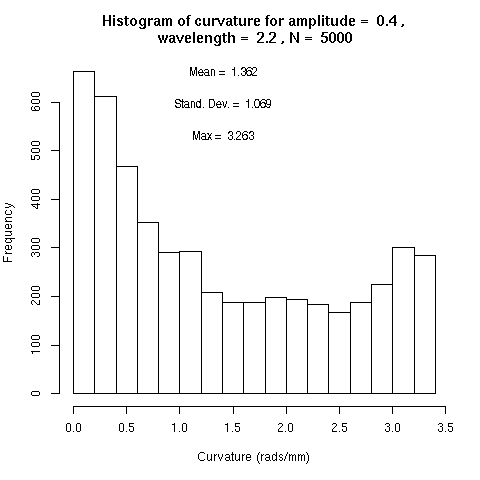
\includegraphics[width=1.0\textwidth]{figcurvhist.png}
%   curvhist.png is original 
  \caption{Simulated histogram of intrinsic curvatures at 5000 points sampled at random along a sine wave of amplitude 0.4 mm over the interval 0 to $2 * \pi$ radians. Curvatures in radians per mm. Mean and standard deviation calculated from histogram data.}
  \label{fig:curvhist}
\end{figure}

%\end{document}

